\documentclass[10pt,aspectratio=169]{beamer}
\usetheme{metropolis}
\usepackage[utf8]{inputenc}
\usepackage[T1]{fontenc}
\usepackage{amsmath,amssymb,bm,mathtools}
\usepackage{graphicx}
\usepackage{booktabs}
\usepackage{subcaption}
\usepackage{capt-of}
\setbeamertemplate{caption}[numbered]
\graphicspath{{chapters/figs/}}

\title{Direction of Arrival (DOA) Estimation}
\subtitle{Signal Models, Preprocessing, Model-Order Selection, and the ESPRIT Family}
\author{Mohammad Raziei}
\date{}

\newcommand{\bx}{\bm{x}}
\newcommand{\bs}{\bm{s}}
\newcommand{\bn}{\bm{n}}
\newcommand{\bA}{\bm{A}}
\newcommand{\ba}{\bm{a}}
\newcommand{\bR}{\bm{R}}
\newcommand{\bI}{\bm{I}}
\newcommand{\bPhi}{\bm{\Phi}}
\newcommand{\bPsi}{\bm{\Psi}}
\newcommand{\bJ}{\bm{J}}
\newcommand{\bPi}{\bm{\Pi}}
\newcommand{\bE}{\bm{E}}
\newcommand{\bT}{\bm{T}}
\newcommand{\bX}{\bm{X}}
\newcommand{\bZ}{\bm{Z}}
\newcommand{\be}{\bm{e}}

\begin{document}

\maketitle

\begin{frame}{Outline}
\tableofcontents
\end{frame}

\section{Motivation and Smart Antenna Systems}

\begin{frame}{Why Estimate Direction of Arrival?}
\begin{itemize}
	\item Wireless applications --- environmental monitoring, sensor networks, public safety, search-and-rescue --- require accurate \textbf{source localization}.
	\item The FCC mandates wireless emergency call location accuracy of \textbf{125 meters}.
	\item DOA estimation of multiple radio wavefronts impinging on a sensor array is central to \textbf{radar, sonar, seismology}, and \textbf{smart antenna} systems.
	\item \textbf{Smart antenna}: multiple antenna elements + signal processing that automatically optimizes the radiation/reception pattern in response to the signal environment.
	\item Benefits: extended coverage range, increased system capacity, and \textbf{Spatial Division Multiple Access (SDMA)} --- multiple users share the same time/frequency resource if spatially separable.
\end{itemize}
\end{frame}

\begin{frame}{Smart Antenna Strategies}
		\centering
\begin{minipage}{.51\linewidth}
\begin{itemize}
	\item \textbf{Switched Lobe (SL)}: switches among a fixed set of predefined beams; selects the one giving the best received power.
	\item \textbf{Phased Array (PA)}: continuously tracks sources using a DOA algorithm; transmission is steered based on estimated angles. A generalization of switched-lobe.
	\item \textbf{Adaptive Array (AA)}: estimates DOA of \emph{both} the desired source and interferers; the beam pattern places nulls toward interference while maximizing gain toward the desired source.
\end{itemize}
	\end{minipage}
	\hfill
	\raisebox{-2.5cm}{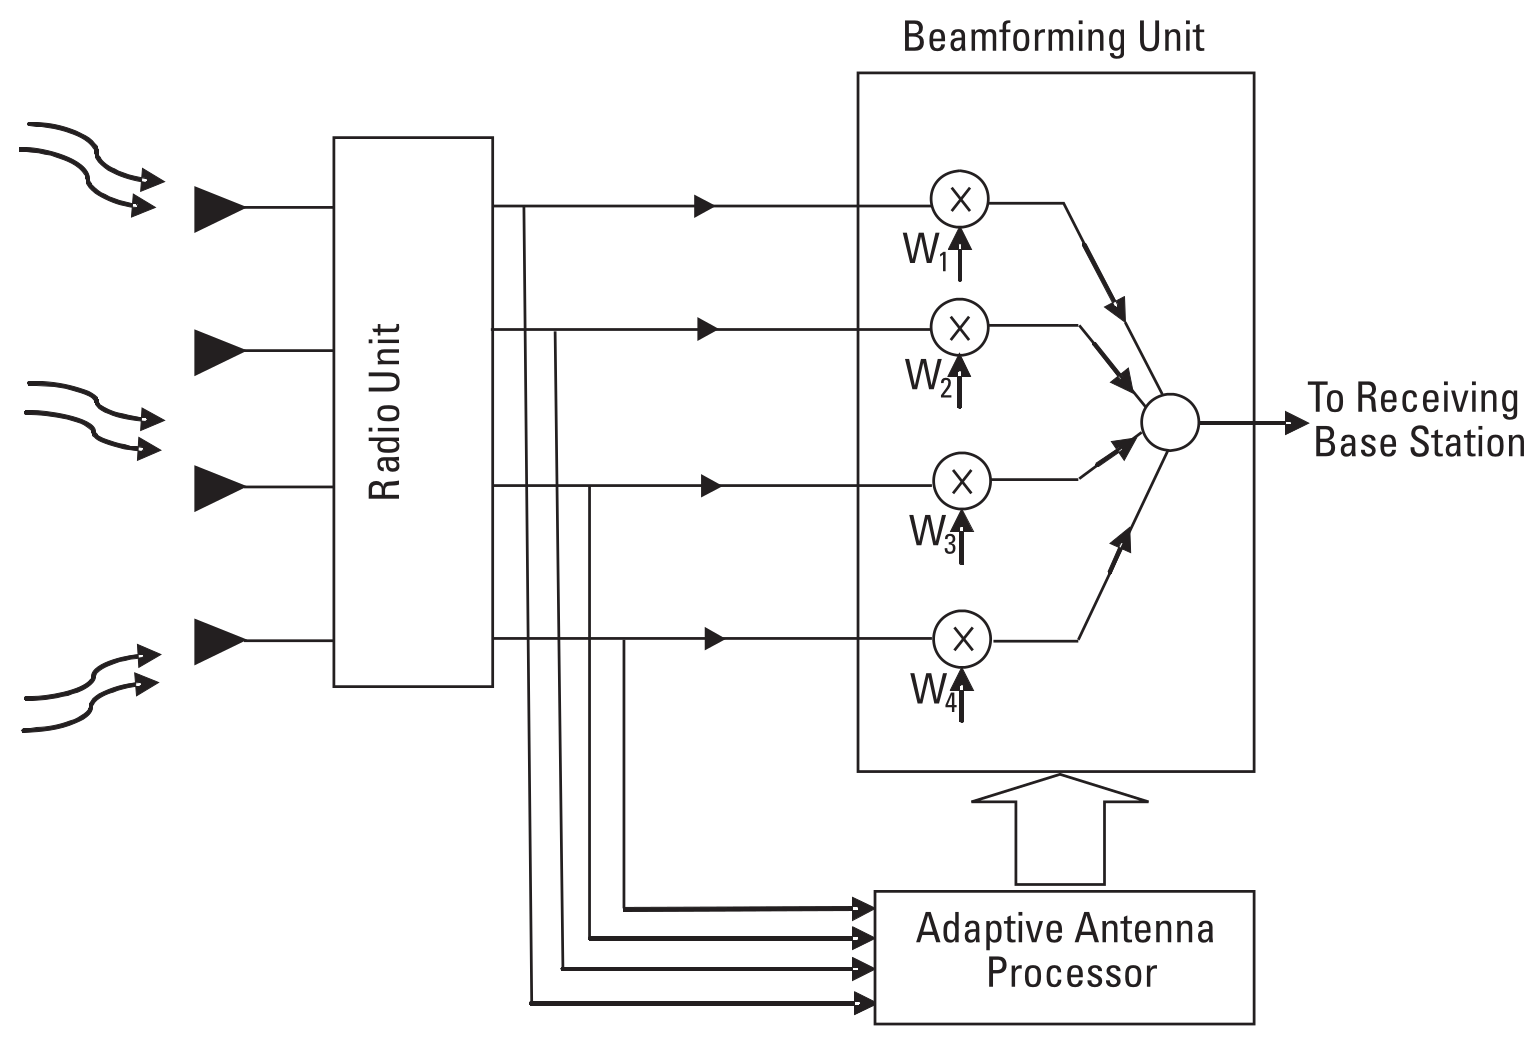
\includegraphics[width=0.45\linewidth]{fig-1-1}}
\end{frame}

\begin{frame}{Adaptive Antenna Processor Architecture}
\centering
\begin{minipage}{.61\linewidth}
	
\begin{itemize}\footnotesize
	\item \textbf{Model order estimator}: estimates the number of impinging wavefronts $d$ (e.g., AIC, MDL) --- required \emph{before} DOA estimation.
	\item \textbf{DOA estimator}: MUSIC, ESPRIT, etc. Subspace tracking (PAST, dPAST) can replace repeated full subspace computation.
	\item \textbf{Spatial filter}: signal reconstruction $\bs = \bm{W}\bX$, with $\bm{W}$ the Moore--Penrose pseudo-inverse of the estimated steering matrix $\hat{\bA}$.
	\item \textbf{User identification, tracking, weight generation}: complete the adaptive beamforming loop.
\end{itemize}

	\end{minipage}
	\hfill
\raisebox{-2.5cm}{
	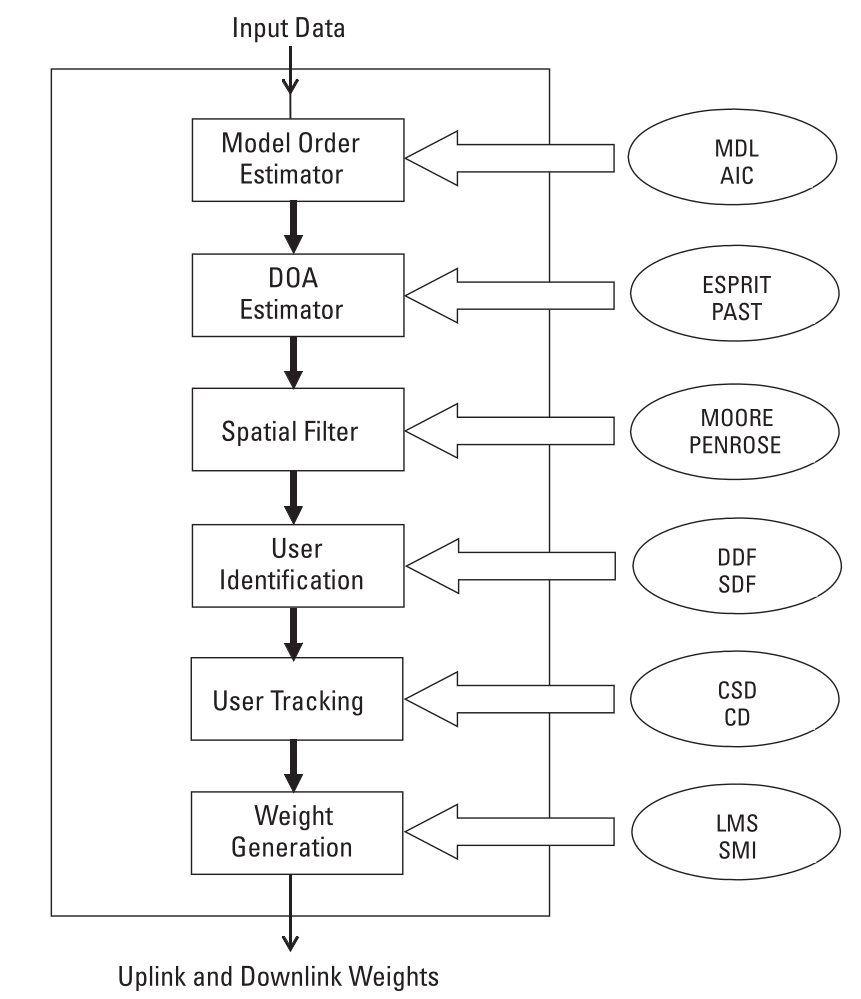
\includegraphics[width=0.36\linewidth]{fig-1-2}}

\end{frame}

\begin{frame}{Beamforming --- the Core Operation}
The beamformer output for a look direction $\theta_i$ is a weighted sum of element outputs:
\begin{equation}
	y(\theta_i) = \sum_{k=0}^{M-1} w_k^i \, x_k
	\label{eq:1-1}
\end{equation}
where $x_k$ is the data sample at element $k$, and $w_k^i$ is the complex weight steering the array toward $\theta_i$ (or nulling it). Choosing $\{w_k\}$ appropriately implements beam steering, adaptive nulling, and beam shaping --- but \emph{which} $\theta_i$ to steer toward is exactly the DOA estimation problem.
\end{frame}

\section{Signal and Data Model}

\begin{frame}{Scenario and Assumptions}
Throughout, we assume:
\begin{itemize}
	\item \textbf{Isotropic, linear propagation medium}: $d$ sources radiate $d$ signals onto an $M$-element sensor array; unit element gain.
	\item \textbf{Far-field assumption}: sources are far enough that wavefronts arrive as \emph{plane waves}. Rule of thumb: range $> 2D^2/\lambda$ ($D$ = array aperture).
	\item \textbf{Narrowband assumption}: all $d$ signals share carrier frequency $f_c$; envelope and phase vary slowly relative to the array transit time $\tau$.
	\item \textbf{AWGN channel}: additive, zero-mean, spatially white noise, uncorrelated with the signals, common variance $\sigma_N^2$ at every element.
\end{itemize}
\end{frame}

\begin{frame}{Narrowband Signal Representation}
Each source's radiated signal:
\begin{equation}
	s_i^r(t) = \alpha_i(t)\cos[2\pi f_c t + \beta_i(t)], \quad 1 \le i \le d
	\label{eq:3-1}
\end{equation}
is narrowband provided $\alpha_i(t-\tau)\approx \alpha_i(t)$ and $\beta_i(t-\tau)\approx\beta_i(t)$. Its \textbf{complex envelope (phasor)}:
\begin{equation}
	s_i(t) = \alpha_i(t)e^{j\beta_i(t)}, \qquad s_i^r(t) = \mathrm{Re}\{s_i(t)e^{j2\pi f_c t}\}
	\label{eq:3-3}
\end{equation}
is the natural representation for array processing, matching how I/Q receivers actually digitize the signal.
\end{frame}

\begin{frame}{ULA Wavefront Geometry}
Consider a Uniform Linear Array (ULA) of $M$ isotropic elements, spacing $\Delta$. A plane wave from angle $\theta_i$ reaches element $m$ with extra path length (relative to element 1):
\begin{equation}
	\Delta_{mi} = (m-1)\Delta\sin\theta_i, \qquad \tau_{mi} = \frac{\Delta_{mi}}{c}
	\label{eq:3-5}
\end{equation}
The phasor received at element $m$ is a phase-shifted copy of that at element 1:
\begin{equation}
	s_{im}(t) \approx s_{i1}(t)\,e^{-j(m-1)\mu_i}
	\label{eq:3-8}
\end{equation}
where the \textbf{spatial frequency} is
\begin{equation}
	\mu_i = \frac{2\pi\Delta}{\lambda}\sin\theta_i .
\end{equation}
DOA estimation $\equiv$ estimating $\mu_i$ from the array data, then inverting $\theta_i = \arcsin(\lambda\mu_i/2\pi\Delta)$.
\end{frame}

\begin{frame}{The Steering Vector}
\textbf{Definition.} The \emph{steering vector} $\ba(\mu_i)\in\mathbb{C}^M$ collects the relative phase shifts seen by every array element for a wavefront with spatial frequency $\mu_i$ (equivalently, angle $\theta_i$):
\begin{equation}
	\ba(\mu_i) = \big[\,1,\; e^{-j\mu_i},\; e^{-j2\mu_i},\; \dots,\; e^{-j(M-1)\mu_i}\,\big]^T, \qquad 1\le i \le d
	\label{eq:3-20}
\end{equation}
\begin{itemize}
	\item It is the array's \emph{spatial impulse response} to a single unit-amplitude plane wave from direction $\theta_i$: entry $m$ is exactly the phase (and, more generally, gain) with which that wavefront appears at sensor $m$.
	\item Stacking the steering vectors of all $d$ sources gives the \textbf{array (steering) matrix}
	\[
	\bA = [\ba(\mu_1), \ba(\mu_2), \dots, \ba(\mu_d)] \in \mathbb{C}^{M\times d},
	\]
	which for a ULA has \textbf{Vandermonde structure} (Eq.~\ref{eq:3-21}).
	\item Every subspace-based DOA algorithm (MUSIC, ESPRIT, \dots) is ultimately a search for which $\ba(\mu)$ (or which subspace) is consistent with the measured covariance.
\end{itemize}
\end{frame}

\begin{frame}{Array Steering Matrix and Data Model}
\begin{equation}
	\bA = [\ba(\mu_1),\dots,\ba(\mu_d)] =
	\begin{bmatrix}
		1 & 1 & \cdots & 1 \\
		e^{-j\mu_1} & e^{-j\mu_2} & \cdots & e^{-j\mu_d}\\
		\vdots & \vdots & \ddots & \vdots \\
		e^{-j(M-1)\mu_1} & e^{-j(M-1)\mu_2} & \cdots & e^{-j(M-1)\mu_d}
	\end{bmatrix}
	\label{eq:3-21}
\end{equation}
Collecting all elements and all sources, the array output vector is
\begin{equation}
	\bx(t) = \sum_{i=1}^d \ba(\mu_i)\, s_i(t) + \bn(t) = \bA\, \bs(t) + \bn(t)
	\label{eq:3-9}
\end{equation}
and the \textbf{data covariance matrix} is
\begin{equation}
	\bR_{xx} = E\{\bx(t)\bx^H(t)\} = \bA\,\bR_{ss}\,\bA^H + \sigma_N^2 \bI_M
	\label{eq:4-1}
\end{equation}
This decomposition into a signal term $\bA\bR_{ss}\bA^H$ (rank $d$, if $\bR_{ss}$ is full rank) plus scaled identity noise is the foundation of every subspace method.
\end{frame}

\begin{frame}{Ambiguity and Spatial Aliasing}
For a unique mapping $\mu_i \leftrightarrow \theta_i$, we require $\mu_i \in [-\pi,\pi]$, restricting DOAs to $[-90^\circ, 90^\circ]$ and requiring
\begin{equation}
	\Delta \le \lambda/2 .
\end{equation}
If violated, a single $\mu_i$ corresponds to two distinct angles $\Rightarrow$ \textbf{grating lobes} appear, admitting signals from unintended directions --- the spatial analogue of violating the Nyquist sampling rate in time.
\end{frame}

\section{Array Geometries: ULA and URA}

\begin{frame}{Centro-Symmetric Arrays}
\textbf{Definition.} An $M$-element array is \emph{centro-symmetric} if its elements are symmetric about a centroid and paired elements have identical radiation characteristics. Then the steering matrix satisfies
\begin{equation}
	\bPi_M \bar{\bA} = \bA \bm{\Lambda}
	\label{eq:3-19}
\end{equation}
with $\bPi_M$ the $M\times M$ exchange (reversal) matrix and $\bm{\Lambda}$ a unitary diagonal matrix. This property underlies \textbf{forward-backward averaging} and the real-valued \textbf{Unitary} transforms used later.

For a centered ULA:
\begin{equation}
	\bPi_M \bar{\bA} = \bA \bm{\Lambda}_\mu, \qquad
	\bm{\Lambda}_\mu = \mathrm{diag}\big(e^{j(M-1)\mu_1},\dots,e^{j(M-1)\mu_d}\big)
	\label{eq:3-22}
\end{equation}
\end{frame}

\begin{frame}{Uniform Rectangular Array (URA)}
For 2-D DOA estimation (azimuth $\phi_i$ and elevation $\theta_i$), a $M_x\times M_y$ URA is used. Define the direction cosines
\begin{equation}
	u_i = \cos\phi_i\sin\theta_i, \qquad v_i = \sin\phi_i\sin\theta_i, \qquad \xi_i = u_i + jv_i
	\label{eq:3-26}
\end{equation}
Then angles are recovered from $\xi_i$ by
\begin{equation}
	\phi_i = \arg(\xi_i), \qquad \theta_i = \arcsin(|\xi_i|)
	\label{eq:3-27}
\end{equation}
i.e., finding DOA reduces to estimating the pair $(u_i, v_i)$ --- one spatial frequency per array axis, handled with the 2-D extensions of the same ULA machinery.
\end{frame}

\section{Categories of DOA Estimators}

\begin{frame}{Three Families of DOA Algorithms}
\begin{block}{Conventional Beamforming}
Scan a beamformer over all angles; the DOA estimates are the angles maximizing output power (e.g., Bartlett, Capon/MVDR). Simple, robust, but limited resolution (Rayleigh limit).
\end{block}
\begin{block}{Subspace-Based Methods}
Decompose $\bR_{xx}$ into orthogonal \emph{signal} and \emph{noise} subspaces (eigendecomposition). MUSIC searches the noise subspace for nulls; ESPRIT exploits an invariance structure directly, avoiding any spectral search. Super-resolution: can separate sources closer than a beamwidth.
\end{block}
\begin{block}{Maximum Likelihood (ML)}
Optimize a likelihood function derived from the assumed statistical data model. Best statistical accuracy, especially at low SNR and few snapshots, at high computational cost (multidimensional nonlinear optimization).
\end{block}
\end{frame}

\section{The Coherent-Signal Problem and Preprocessing}

\begin{frame}{Why Preprocessing Is Needed}
Subspace algorithms require $\bR_{ss}$ full rank ($=d$). If two wavefronts are \textbf{coherent} (e.g., multipath: $s_2(t)=\alpha s_1(t)$), then
\begin{equation}
	\bs(t) = [s_1(t), \alpha s_1(t), s_3(t), \dots, s_d(t)]^T
	\label{eq:4-2}
\end{equation}
makes $\bR_{ss}$ singular. Consequences:
\begin{enumerate}
	\item The multiplicity of the smallest eigenvalue of $\bR_{xx}$ becomes $k=M-d+1$ (instead of $M-d$) $\Rightarrow$ the number of sources is under-estimated as $d-1$.
	\item Only $d-1$ directions remain separable.
\end{enumerate}
This is common in multipath-rich environments. \textbf{Solution}: decorrelating preprocessing before running any DOA algorithm.
\end{frame}

\begin{frame}{Forward--Backward (FB) Averaging}
Applicable to centro-symmetric arrays. Key identity for a ULA:
\begin{equation}
	\bPi_M \bar{\ba}(\theta_i) = e^{-j(M-1)\mu_i}\ba(\theta_i)
	\label{eq:4-4}
\end{equation}
Form the backward covariance $\bR_{back} = \bPi_M \bar\bR_{xx} \bPi_M$ and average:
\begin{equation}
	\bR_{xx}^{fb} = \tfrac12\big(\bR_{xx} + \bPi_M \bar\bR_{xx}\bPi_M\big)
	= \bA\Big[\tfrac12(\bR_{ss}+\bm{\Delta}\bar\bR_{ss}\bm{\Delta}^H)\Big]\bA^H + \sigma_N^2\bI_M
	\label{eq:4-6}
\end{equation}
The new signal covariance $\bR_{ss}^{fb}=\tfrac12(\bR_{ss}+\bm\Delta\bar\bR_{ss}\bm\Delta^H)$ has rank $d$ \emph{even for fully coherent sources}. In practice, using data matrix $\bZ=[\bX,\,\bPi_M\bar\bX]\in\mathbb{C}^{M\times 2N}$:
\begin{equation}
	\hat\bR_{xx}^{fb} = \frac{1}{2N}\bZ\bZ^H
	\label{eq:4-9}
\end{equation}
FB averaging is built into Unitary ESPRIT automatically (Section~\ref{sec:unitary-esprit-slide}).
\end{frame}

\begin{frame}{Spatial Smoothing --- 1-D}
Handles \emph{more than two} coherent sources, where FB averaging alone is insufficient. Split the $M$-element ULA into $L$ overlapping subarrays of $M_{sub}=M-L+1$ elements each (Fig.~\ref{fig:4-1}).
\begin{columns}
\begin{column}{0.48\textwidth}
\begin{equation}
	\bJ_l^{(M)} = [\bm{0}\;\; \bI_{M_{sub}} \;\;\bm{0}], \quad 1\le l \le L
	\label{eq:4-10}
\end{equation}
\begin{equation}
	\bX_l = \bJ_l^{(M)}\bX = \bA_1\bPhi^{l-1}\bs + \bJ_l^{(M)}\bn
	\label{eq:4-11}
\end{equation}
\end{column}
\begin{column}{0.48\textwidth}
	\centering
	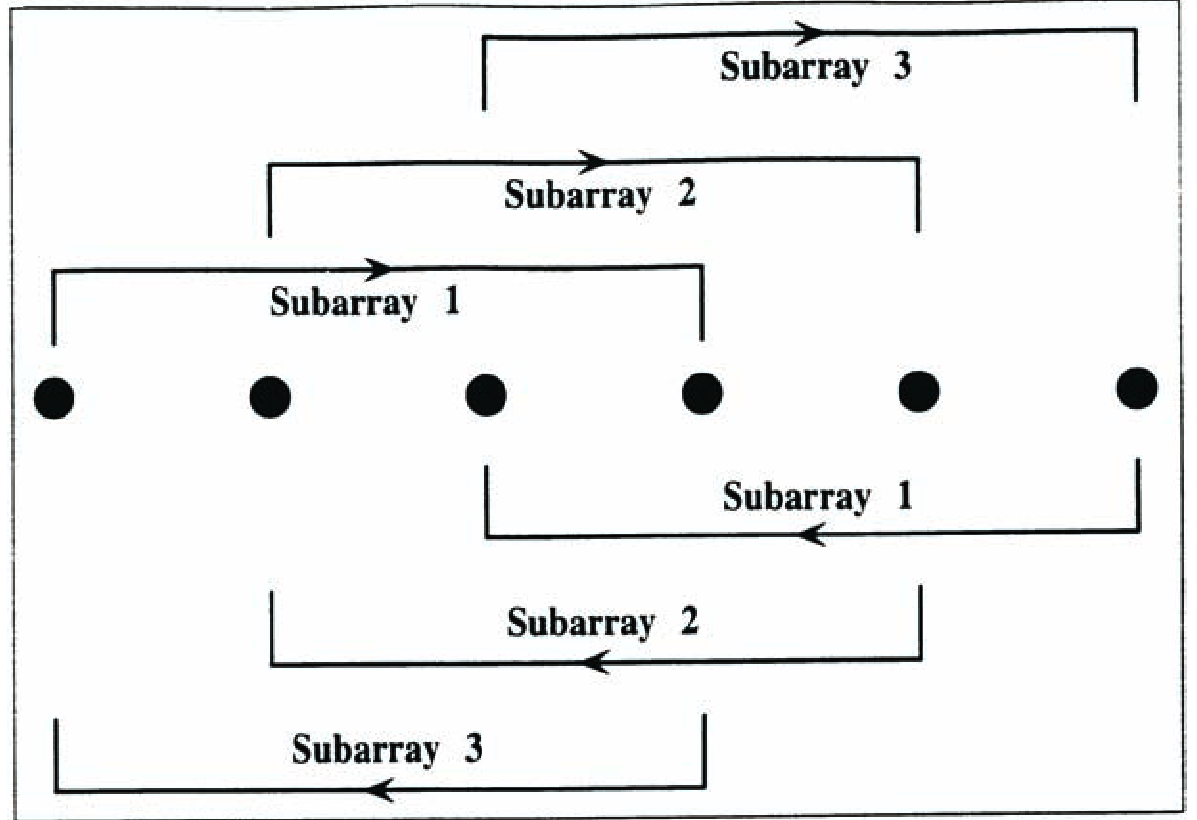
\includegraphics[width=\linewidth]{fig-4-1}
	\captionof{figure}{\footnotesize Forward/backward subarrays for 1-D smoothing.}
	\label{fig:4-1}
\end{column}
\end{columns}
\end{frame}

\begin{frame}{Spatial Smoothing --- Averaged Covariance}
Averaging the subarray covariances:
\begin{equation}
	\bR_{xx}^{ss} = \frac1L\sum_{l=1}^L \bJ_l^{(M)}\bR_{xx}\bJ_l^{(M)T}
	= \bA_1\Big(\underbrace{\tfrac1L\sum_{l=1}^L \bPhi^{l-1}\bR_{ss}\bar\bPhi^{l-1}}_{\bR_{ss}^{ss}}\Big)\bA_1^H + \sigma^2\bI_{M_{sub}}
	\label{eq:4-14}
\end{equation}
\begin{itemize}
	\item $\bR_{ss}^{ss}$ regains full rank $d$ even when $L$ signals are mutually coherent.
	\item \textbf{Cost}: effective aperture shrinks from $M$ to $M_{sub}$; snapshots effectively increase from $N$ to $NL$.
	\item Minimum elements needed: $M_{sub}=d+1$ per subarray (vs.\ $d+1$ total for uncorrelated signals).
	\item \textbf{Forward-backward spatial smoothing} (averaging both directions) reduces the requirement further to $M \approx 3d/2$.
\end{itemize}
\end{frame}

\begin{frame}{Spatial Smoothing --- Simulation Evidence}
\centering
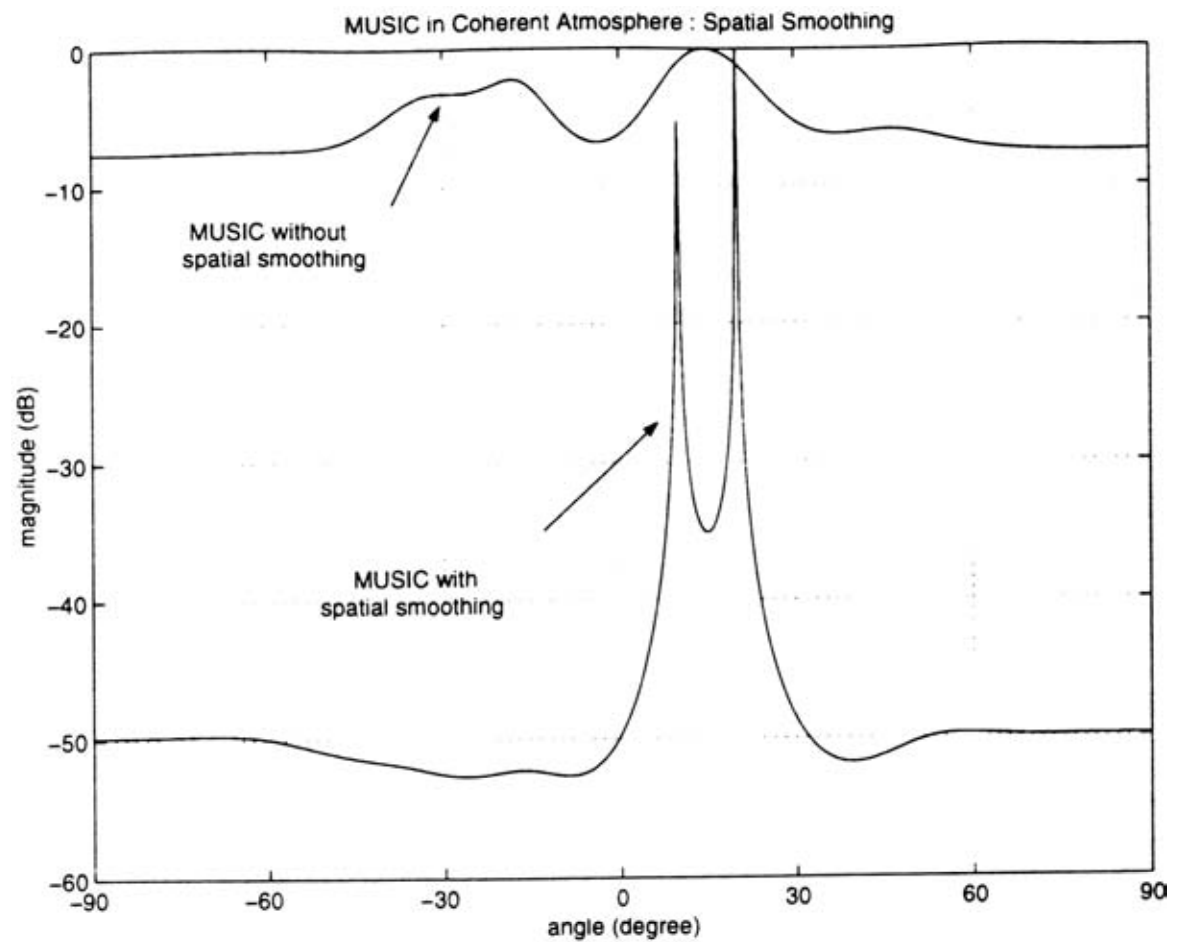
\includegraphics[width=0.85\linewidth]{fig-4-2}
\captionof{figure}{\footnotesize MUSIC pseudo-spectrum with/without spatial smoothing: two coherent sources at $10^\circ$ and $20^\circ$, 6-element ULA, SNR $=20$\,dB. Conventional MUSIC fails completely; smoothed MUSIC clearly resolves both peaks.}
\end{frame}

\begin{frame}{Spatial Smoothing --- 2-D (URA)}
The URA is treated as ULAs along $x$ and $y$; 1-D smoothing selection matrices combine via the \textbf{Kronecker product}:
\begin{equation}
	\bJ_{l_x,l_y} = \bJ_{l_y}^{(M_y)} \otimes \bJ_{l_x}^{(M_x)}, \quad 1\le l_x\le L_x,\; 1\le l_y \le L_y
	\label{eq:4-17}
\end{equation}
\begin{columns}
\begin{column}{0.5\textwidth}
Example: $M=4\times5$ URA, $L_x=2, L_y=3 \Rightarrow$ $L=6$ rectangular subarrays, each with $M_{sub}=3\times3=9$ elements.
\begin{equation}
	\bX_{ss}=[\bJ_{1,1}\bX\;\cdots\;\bJ_{L_x,L_y}\bX]\in\mathbb{C}^{M_{sub}\times NL}
	\label{eq:4-18}
\end{equation}
\end{column}
\begin{column}{0.3\textwidth}
	\centering
	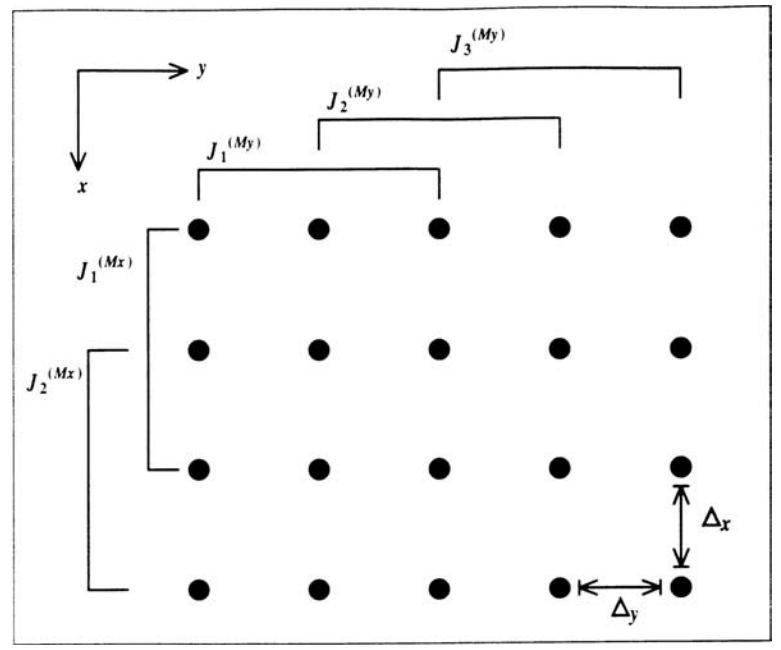
\includegraphics[width=\linewidth]{fig-4-3}
	\captionof{figure}{\footnotesize 2-D spatial smoothing subarrays.}
\end{column}
\end{columns}
This 2-D smoothing precedes 2-D ESPRIT when coherent sources are present.
\end{frame}

\section{Model Order Estimation}

\begin{frame}{How Many Signals? The Classical (Eigenvalue) Method}
DOA algorithms must know $d$ in advance. Since
\begin{equation}
	\bR_{xx} = E\{\bx(t)\bx^H(t)\} = \bA\bR_{ss}\bA^H + \sigma_N^2\bI_M
	\label{eq:4-19}
\end{equation}
theoretically has $M-d$ small eigenvalues all equal to $\sigma_N^2$, the number of sources follows from the multiplicity $k$ of the smallest eigenvalue:
\begin{equation}
	d = M-k
	\label{eq:4-20}
\end{equation}
In practice, with finite samples these eigenvalues cluster rather than coincide exactly, motivating statistical detection criteria (MDL, AIC).
\end{frame}

\begin{frame}{Minimum Description Length (MDL)}
Choose $d\in\{0,\dots,M-1\}$ minimizing
\begin{equation}
	\mathrm{MDL}(d) = -\log\left\{\frac{\prod_{i=d+1}^M \lambda_i^{1/(M-d)}}{\frac{1}{M-d}\sum_{i=d+1}^M \lambda_i}\right\}^{(M-d)N} + \hat p(k)\log N
	\label{eq:4-21}
\end{equation}
with penalty term
\begin{equation}
	\hat p(k)=
	\begin{cases}
		d(2M-d+1) & \text{real matrices}\\
		d(M+d+1) & \text{real FB averaging}\\
		d(2M-d) & \text{complex matrices}\\
		0.5\,d(2M-d+1) & \text{complex FB averaging}
	\end{cases}
	\label{eq:4-22}
\end{equation}
Max detectable order: $d_{\max}=\min\{M,N\}$ (ULA) or $\min\{M_xM_y, N\}$ (URA).
\end{frame}

\begin{frame}{MDL --- Simulation Results}
\centering
\begin{columns}
\begin{column}{0.45\textwidth}
	\centering
	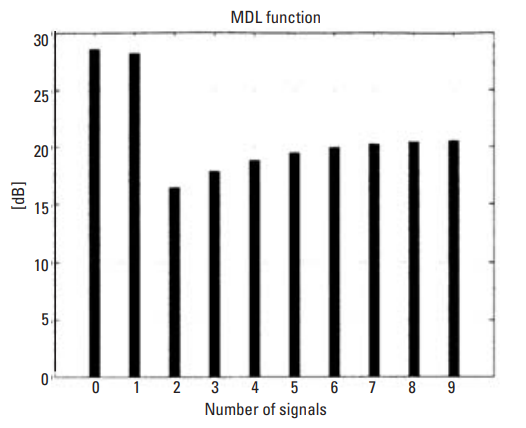
\includegraphics[width=\linewidth]{fig-4-4-a}
	\captionof{figure}{\footnotesize Two coherent signals}
\end{column}
\begin{column}{0.45\textwidth}
	\centering
	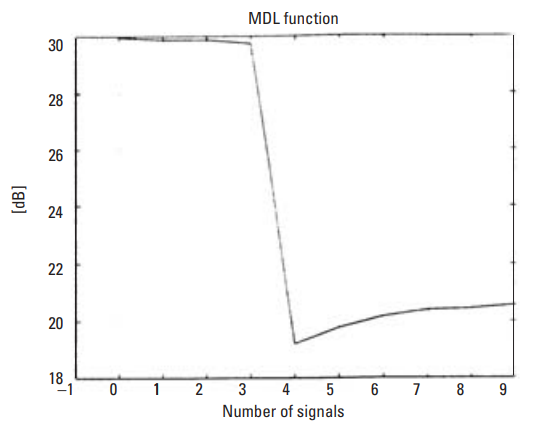
\includegraphics[width=\linewidth]{fig-4-4-b}
	\captionof{figure}{\footnotesize Four coherent signals}
\end{column}
\end{columns}
\vspace{2mm}
10-element ULA, SNR $=0$\,dB, 50 trials $\times$ 250 snapshots. MDL correctly identifies 2 and 4 sources, respectively.
\end{frame}

\begin{frame}{Akaike Information Criterion (AIC)}
Similar structure, different penalty:
\begin{equation}
	AIC(d) = -\log\left\{\frac{\prod_{i=d+1}^M \lambda_i^{1/(M-d)}}{\frac{1}{M-d}\sum_{i=d+1}^M \lambda_i}\right\}^{(M-d)N} + \hat p(k)
	\label{eq:4-25}
\end{equation}
where $\hat p(k)$ uses the same four cases as MDL but \emph{without} the $\log N$ scaling. AIC tends to slightly over-estimate model order relative to MDL, but is asymptotically less biased for small samples in some regimes.
\end{frame}

\begin{frame}{AIC --- Simulation Results}
\centering
\begin{columns}
\begin{column}{0.5\textwidth}
	\centering
	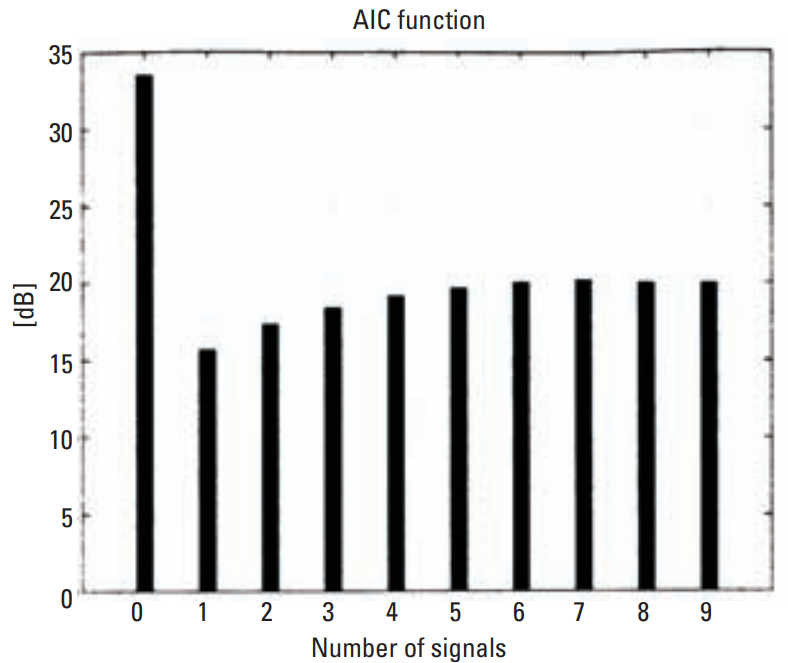
\includegraphics[width=\linewidth]{fig-4-5-a}
	\captionof{figure}{\footnotesize Two impinging signals}
\end{column}
\begin{column}{0.5\textwidth}
	\centering
	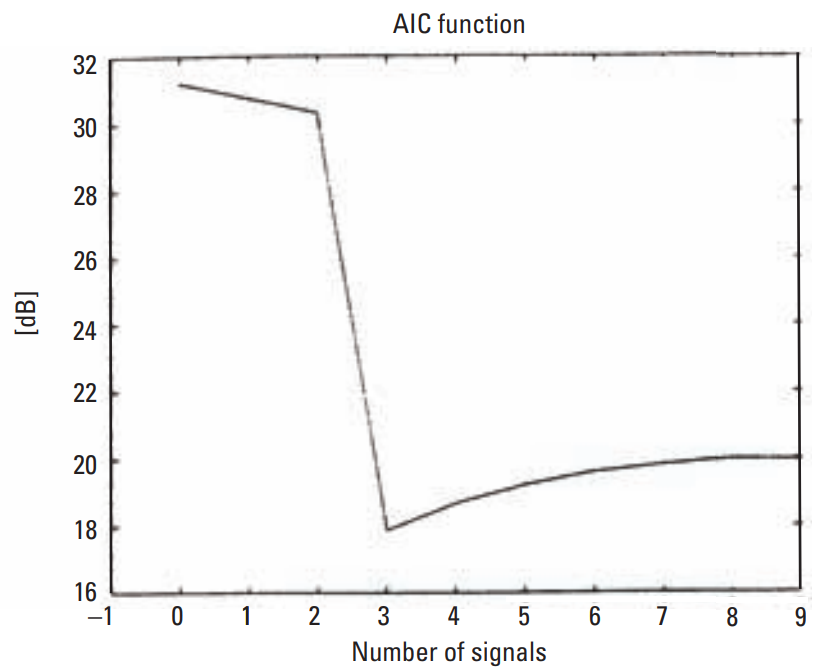
\includegraphics[width=\linewidth]{fig-4-5-b}
	\captionof{figure}{\footnotesize Three impinging signals}
\end{column}
\end{columns}
\vspace{2mm}
Same ULA/SNR setup as before; AIC's minimum lands exactly at the true number of sources in each case.
\end{frame}

\section{ESPRIT: Estimation of Signal Parameters via Rotational Invariance}

\begin{frame}{Why ESPRIT?}
Spectral methods (MUSIC, beamforming) require:
\begin{itemize}
	\item precise knowledge of the array manifold $\bA(\theta)$ (calibration-sensitive, expensive), and
	\item an exhaustive search over all candidate angles/steering vectors --- computationally heavy.
\end{itemize}
\textbf{ESPRIT} exploits a built-in \emph{shift-invariance} of the array to avoid both: no manifold knowledge, no spectral search, and drastically reduced computation and memory.
\end{frame}

\begin{frame}{ESPRIT Array Structure}
\centering
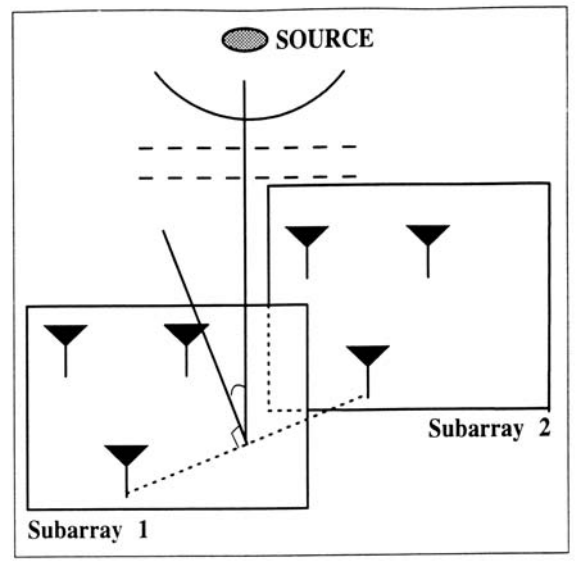
\includegraphics[width=0.5\linewidth]{fig-5-1}
\captionof{figure}{\footnotesize Two identical, displaced subarrays (``doublets'') --- the structural requirement for ESPRIT.}
\vspace{2mm}

Two identical subarrays, each with $m$ elements, related by a fixed \textbf{displacement vector} $\Delta$. Overlap allowed ($M\le 2m$) or not ($M=2m$). Each sensor pair (doublet) can have arbitrary but matched gain/phase/polarization.
\end{frame}

\begin{frame}{ESPRIT Signal Model}
With subarray outputs $\bx_1(t),\bx_2(t)$:
\begin{subequations}
\begin{align}
	\bx_1(t) &= \bA\bs(t) + \bn_1(t) \label{eq:5-1a}\\
	\bx_2(t) &= \bA\bPhi\,\bs(t) + \bn_2(t) \label{eq:5-1b}
\end{align}
\end{subequations}
where $\bPhi = \mathrm{diag}[e^{j\mu_1},\dots,e^{j\mu_d}]$ is the \textbf{rotation operator} encoding the extra phase delay caused by the fixed subarray displacement $\Delta$:
\[ \mu_i = -\tfrac{2\pi}{\lambda}\Delta\sin\theta_i . \]
Stacking:
\begin{equation}
	\bx(t) = \begin{bmatrix}\bx_1(t)\\ \bx_2(t)\end{bmatrix}
	= \begin{bmatrix}\bA\\ \bA\bPhi\end{bmatrix}\bs(t) + \begin{bmatrix}\bn_1(t)\\\bn_2(t)\end{bmatrix}
	= \tilde\bA\bs(t) + \bn(t)
	\label{eq:5-2}
\end{equation}
Goal: estimate each $\mu_i$ by determining $\bPhi$.
\end{frame}

\begin{frame}{Step 1: Signal Subspace Estimation}
Since $\bR_{xx}=E\{\bx(t)\bx^H(t)\} = \tilde\bA\bR_{ss}\tilde\bA^H$ (Eq.~\ref{eq:5-3}) with $\bR_{ss}, \tilde\bA$ full rank $d$, the signal subspace $\bE_s=[\be_1,\dots,\be_d]$ (top $d$ eigenvectors) spans the same range as $\tilde\bA$:
\[ \bE_s = \tilde\bA\bT \quad\text{for some nonsingular } \bT. \]
Partition $\bE_s$ into the two subarray blocks:
\begin{equation}
	\bE_s = \begin{bmatrix}\bE_1\\ \bE_2\end{bmatrix} = \begin{bmatrix}\bA\bT\\ \bA\bPhi\bT\end{bmatrix}
	\label{eq:5-4}
\end{equation}
so $\mathrm{Range}\{\bE_1\}=\mathrm{Range}\{\bE_2\}=\mathrm{Range}\{\bA\}$ (Eq.~\ref{eq:5-5}).
\end{frame}

\begin{frame}{Step 2: The Invariance Equation}
Since $\bE_1,\bE_2$ span the same $d$-dimensional space, there exists a nonsingular $d\times d$ matrix $\bPsi$ with
\begin{equation}
	\bE_1\bPsi = \bE_2 \;\Longrightarrow\; \bA\bT\bPsi = \bA\bPhi\bT
	\label{eq:5-6}
\end{equation}
\begin{equation}
	\bPsi = \bT^{-1}\bPhi\bT
	\label{eq:5-7}
\end{equation}
\textbf{Key fact}: $\bPsi$ and $\bPhi$ are related by an eigenvalue-preserving similarity transform $\Rightarrow$ the eigenvalues of $\bPsi$ \emph{are exactly} the diagonal entries of $\bPhi$, i.e., $e^{j\mu_i}$.

So ESPRIT never needs $\bA(\theta)$ itself: it solves the small $d\times d$ eigenproblem for $\bPsi$, obtained purely from the signal subspace, and reads off $\mu_i$ from its eigenvalues.
\end{frame}

\begin{frame}{Step 3: Estimating $\bPsi$ --- LS vs.\ TLS}
In practice $\bE_s$ is estimated from noisy finite data, so $\bE_1\bPsi=\bE_2$ has no exact solution. Treat it as $\bm{A}_{\text{eq}}\bm{X}=\bm{B}_{\text{eq}}$:
\begin{itemize}
	\item \textbf{Least Squares (LS)}: assumes $\bE_1$ is exact, all error lies in $\bE_2$:
	\begin{equation}
		\hat\bPsi_{LS} = (\bE_1^H\bE_1)^{-1}\bE_1^H\bE_2
	\end{equation}
	\item \textbf{Total Least Squares (TLS)}: allows errors in \emph{both} $\bE_1$ and $\bE_2$ --- minimizes $\|[\bm{R}_{E_1}\;\bm{R}_{E_2}]\|_F$ subject to $(\bE_1+\bm{R}_{E_1})\hat\bPsi=(\bE_2+\bm{R}_{E_2})$. Generally more accurate since both subarray estimates are noisy. Solved via SVD of $[\bE_1 \; \bE_2]$.
\end{itemize}
These two choices define \textbf{LS-ESPRIT} and \textbf{TLS-ESPRIT}.
\end{frame}

\begin{frame}{Standard ESPRIT on a ULA}
\centering
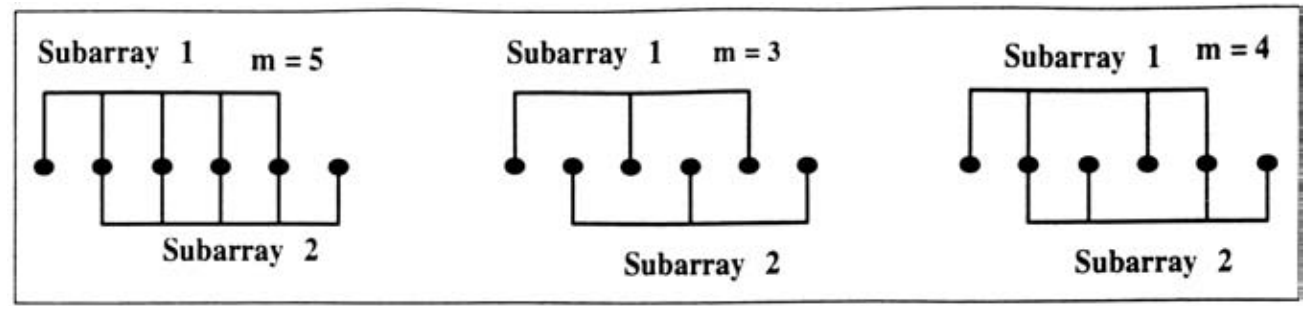
\includegraphics[width=0.95\linewidth]{fig-5-2}
\captionof{figure}{\footnotesize Centro-symmetric linear subarray configurations for ESPRIT.}
\vspace{1mm}
Maximum-overlap selection matrices ($m=M-1$ each):
\begin{equation}
	\bJ_1 = [\bI_m \;\; \bm{0}], \qquad \bJ_2 = [\bm{0}\;\; \bI_m] \in \mathbb{R}^{m\times M}, \qquad \bJ_2 = \bPi_m\bJ_1\bPi_M
	\label{eq:5-9}
\end{equation}
\end{frame}

\begin{frame}{The Invariance Property in Matrix Form}
Because of the fixed shift $\Delta$ between subarrays:
\begin{equation}
	\bJ_2\ba(\mu_i) = e^{j\mu_i}\,\bJ_1\ba(\mu_i), \qquad 1\le i\le d
	\label{eq:5-11}
\end{equation}
or, compactly for all sources at once:
\begin{equation}
	\bJ_1\bA\bPhi = \bJ_2\bA
	\label{eq:5-12}
\end{equation}
This is the shift-invariance identity underlying the entire ESPRIT family. Solving the corresponding equation on the \emph{estimated signal subspace} yields $\hat\bPsi$ and hence
\begin{equation}
	\hat\mu_i = \angle\lambda_i(\hat\bPsi), \qquad \hat\theta_i = \arcsin\!\Big(\frac{-\lambda\,\hat\mu_i}{2\pi\Delta}\Big)
\end{equation}
\end{frame}

\begin{frame}{ESPRIT: Practical Advantages}
\begin{itemize}
	\item No exhaustive angular search --- only an eigen-decomposition of $\bR_{xx}$ and a small $d\times d$ eigenproblem for $\bPsi$.
	\item No array manifold calibration is strictly required (relative to MUSIC).
	\item Naturally extends to 2-D (URA) geometries and to real-valued (\textbf{Unitary}) implementations.
	\item Serves as the algorithmic backbone for many modern high-resolution DOA techniques.
\end{itemize}
\end{frame}

\section{Unitary ESPRIT}
\label{sec:unitary-esprit-slide}

\begin{frame}{Motivation for Real-Valued (Unitary) Processing}
Standard ESPRIT operates on complex-valued matrices: complex EVD/SVD roughly doubles computational cost relative to an equivalent real-valued problem. \textbf{Unitary ESPRIT} applies a unitary transformation exploiting the centro-symmetric structure (Eq.~\ref{eq:3-19}) to convert the complex problem into a fully \textbf{real-valued} one.
\begin{itemize}
	\item Forward--backward averaging is realized \emph{intrinsically} --- no separate FB-averaging step needed.
	\item Real eigen-decompositions are numerically more stable and roughly $4\times$ cheaper than the complex equivalent.
	\item Extends to 1-D and 2-D (element-space and beamspace) formulations.
\end{itemize}
\end{frame}

\begin{frame}{Unitary ESPRIT --- Element Space (1-D)}
The real-valued invariance equation replacing Eq.~\ref{eq:5-12} takes the form
\[
	\bm{K}_1 \bm{E}_{s}^{\mathbb{R}} \,\bm\Upsilon = \bm{K}_2 \bm{E}_{s}^{\mathbb{R}}
\]
where $\bm{E}_s^{\mathbb{R}}$ is a \emph{real} signal subspace basis obtained via a unitary similarity transform $\bm{Q}_M^H$ applied to $\bR_{xx}$, and $\bm{K}_1,\bm{K}_2$ are real selection matrices derived from $\bJ_1,\bJ_2$. The eigenvalues of the resulting real matrix $\bm\Upsilon$ are related to $\mu_i$ by
\[
	\mu_i = 2\arctan(\lambda_i(\bm\Upsilon))
\]
(a Cayley-type transform), avoiding complex arithmetic throughout.
\end{frame}

\begin{frame}{Unitary ESPRIT --- 2-D and Beamspace}
\begin{itemize}
	\item \textbf{2-D Unitary ESPRIT (element space)}: applies the same real-valued transform along both array axes of a URA, jointly estimating $(u_i,v_i)$; includes an automatic pairing step to match azimuth/elevation estimates belonging to the same source.
	\item \textbf{DFT beamspace transform}: projects element-space data onto a small set of orthogonal beams (via a DFT matrix) before applying ESPRIT, exploiting the inherent shift-invariance of the DFT beamspace manifold; reduces dimensionality and computational load further.
	\item \textbf{Unitary ESPRIT in DFT beamspace}: combines both ideas --- real-valued and reduced-dimension --- for the most computationally efficient variant discussed in the source material.
\end{itemize}
\end{frame}

\section{Summary}

\begin{frame}{Summary}
\begin{itemize}
	\item DOA estimation extracts the spatial frequency $\mu_i$ (hence angle $\theta_i$) of each impinging wavefront from array data $\bx(t)=\bA\bs(t)+\bn(t)$, where every column of $\bA$ is a \textbf{steering vector} $\ba(\mu_i)$.
	\item Three algorithm families: \textbf{beamforming}, \textbf{subspace-based}, and \textbf{maximum likelihood}.
	\item Before applying any subspace algorithm: (1) resolve \textbf{coherent-signal} rank deficiency via \textbf{FB averaging} / \textbf{spatial smoothing}; (2) determine the \textbf{number of sources} via \textbf{MDL} / \textbf{AIC}.
	\item \textbf{ESPRIT} exploits shift-invariance between two displaced subarrays to estimate DOA \emph{without} a spectral search or manifold calibration --- solved via LS or TLS on the invariance equation.
	\item \textbf{Unitary ESPRIT} recasts the same computation in real arithmetic, with built-in FB averaging, extending naturally to 2-D element-space and DFT-beamspace formulations.
\end{itemize}
\end{frame}

\begin{frame}{References (Source Material)}
\footnotesize
Content adapted and translated from the \emph{DoA Book} (chapters 1--5: Introduction; Array Systems; Basic DOA Algorithms; Preprocessing \& Model-Order Estimation; ESPRIT), including all cited figures. Original key references include M.~Haardt's doctoral work on array signal processing for DOA estimation (Shaker Verlag), and standard treatments of MUSIC, ESPRIT, MDL, and AIC in the array-processing literature.
\end{frame}

\begin{frame}
\centering
\Huge Thank You
\vspace{0.5cm}
\normalsize

\large Questions \& Discussion
\end{frame}

\end{document}
